\documentclass[12pt,letterpaper]{article}

\newenvironment{proof}{\noindent{\bf Proof:}}{\qed\bigskip}

\newtheorem{theorem}{Theorem}
\newtheorem{corollary}{Corollary}
\newtheorem{lemma}{Lemma} 
\newtheorem{claim}{Claim}
\newtheorem{fact}{Fact}
\newtheorem{definition}{Definition}
\newtheorem{assumption}{Assumption}
\newtheorem{observation}{Observation}
\newtheorem{example}{Example}
\newcommand{\qed}{\rule{7pt}{7pt}}

\newcommand{\assignment}[4]{
\thispagestyle{plain} 
\newpage
\setcounter{page}{1}
\noindent
\begin{center}
\framebox{ \vbox{ \hbox to 6.28in
{\bf CS578/STAT590: Introduction Machine Learning \hfill #1}
\vspace{4mm}
\hbox to 6.28in
{\hspace{2.5in}\large\mbox{Problem Set #2}}
\vspace{4mm}
\hbox to 6.28in
{{\it Handed Out: #3 \hfill Due: #4}}
}}
\end{center}
}

\newcommand{\solution}[4]{
\thispagestyle{plain} 
\newpage
\setcounter{page}{1}
\noindent
\begin{center}
\framebox{ \vbox{ \hbox to 6.28in
{\bf CS578/STAT590: Introduction to Machine Learning \hfill #4}
\vspace{4mm}
\hbox to 6.28in
{\hspace{2.5in}\large\mbox{Problem Set #3}}
\vspace{4mm}
\hbox to 6.28in
{#1 \hfill {\it Handed In: #2}}
}}
\end{center}
\markright{#1}
}

\newenvironment{algorithm}
{\begin{center}
\begin{tabular}{|l|}
\hline
\begin{minipage}{1in}
\begin{tabbing}
\quad\=\qquad\=\qquad\=\qquad\=\qquad\=\qquad\=\qquad\=\kill}
{\end{tabbing}
\end{minipage} \\
\hline
\end{tabular}
\end{center}}

\def\Comment#1{\textsf{\textsl{$\langle\!\langle$#1\/$\rangle\!\rangle$}}}



\oddsidemargin 0in
\evensidemargin 0in
\textwidth 6.5in
\topmargin -0.5in
\textheight 9.0in

\begin{document}

\solution{Gen Nishida}{\today}{1}{Fall 2014}
% Fill in the above, for example, as follows:
% \solution{John Smith}{\today}{1}{Fall 2014}

\pagestyle{myheadings}  % Leave this command alone

\section{Review Questions}

\begin{enumerate}
\item Assume the probability of getting {\it head} when tossing a coin is $\lambda$.
\begin{itemize}
\item What is the probability of getting the first head at the (k+1)-th toss?
\[
(1-\lambda)^k \lambda
\]
\item What is the expected number of tosses needed to get the first head?\\
Let $k$ be the number of tosses needed to get the first head. Then the expected number of $k$ is defined by
\begin{eqnarray}
E[k]&=&\lambda \times 1 + (1-\lambda) \lambda \times 2 + (1-\lambda)^2 \lambda \times 2 + \cdots\\
(1-\lambda)E[k]&=&(1-\lambda)\lambda + (1-\lambda)^2 \lambda \times 2 + (1-\lambda)^3 \lambda \times 3 + \cdots
\end{eqnarray}
By subtracting (2) from (1), we get
\begin{eqnarray*}
\lambda E[k] &=& \lambda + (1-\lambda) \lambda + (1-\lambda)^2 \lambda + (1-\lambda)^3 \lambda + \cdots\\
 &=&\lambda \frac{1}{1 - (1 - \lambda)}\\
 &=&1 .
\end{eqnarray*}
Thus, $E[k]=1 / \lambda $.
\end{itemize}

\item Let $f(x, y)=3x^2+y^2-xy-11x$

\begin{itemize}
\item What is the partial derivative of $f$ with respect to $x$ $(\frac{\partial f}{\partial x})$? Find $\frac{\partial f}{\partial y}$ as well.
\[
\frac{\partial f}{\partial x}=6x-y-11,\:\:  \frac{\partial f}{\partial y}=2y - x
\]
\item Find a point $(x, y)$ that minimizes $f$.
\[
\left\{
\begin{array}{l}
6x-y-11=0 \\
2y-x=0
\end{array}
\right.
\]
By solving these equations, we get $(x, y)=(2, 1)$.
\end{itemize}

\item 
\begin{itemize}
\item Assume that $\omega \in R^n$ and $b$ is a scalar. A hyperplane in $\mathbb{R}^n$ is the set $\{x : x\in \mathbb{R}^n, \omega^Tx+b=0\}$. For $n=2$ and $n=3$, draw on paper an example of a hyperplane.\\
The hyperplane has it normal vector $\omega$, and it is away from the origin by $-b/\|\omega\|$. The example of a hyperplane for $n=2$ and $n=3$ is in Figure 1.

\begin{figure}[hbtp]
\caption{Figure 1}
\centering
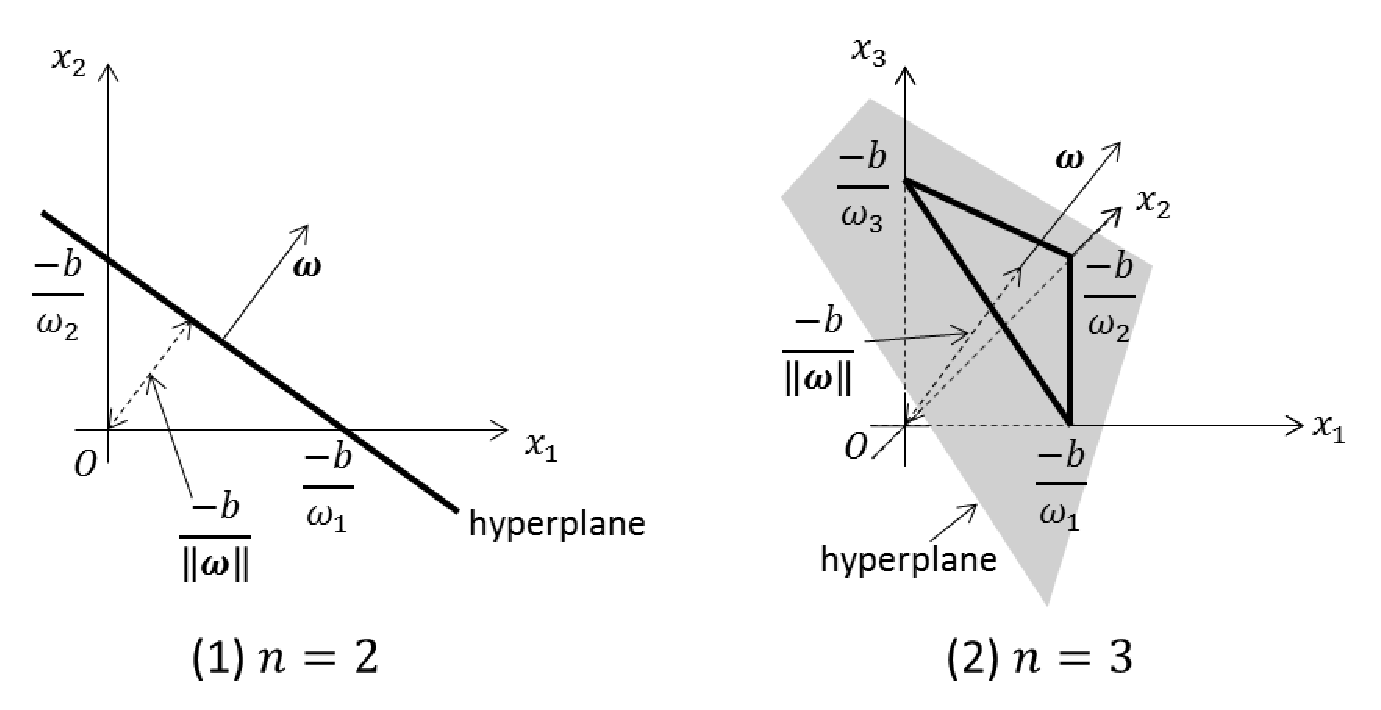
\includegraphics[scale=1]{figure1.eps}
\end{figure}


\item Assume we have two parallel hyperplanes: $\{x: x\in \mathbb{R}^n, \omega^Tx+b_1=0\}$ and $\{x: x\in \mathbb{R}^n, \omega^Tx+b_2=0\}$. What is the distance between these two hyperplanes?
\[
\left|\frac{-b_1}{\|\omega\|}-\frac{-b_2}{\|\omega\|}\right|=\frac{|b_1-b_2|}{\|\omega\|}
\]
\end{itemize}
\end{enumerate}

\section{Basic Concepts}
\begin{enumerate}
\item Define in one sentence: (1) training set, (2) test set, (3) validation set.
\begin{itemize}
\item training set

Training set is a set of data used to optimize a hypothesis function.

\item test set

Test set is a set of real-world data used to measure the accuracy of the hypothesis generated through training and validation phases.

\item validation set

Validation set is a set of data used to estimate the performance of the hypothesis.

\end{itemize}

\item Can you use the validation set as a test set?

No. Since validation set is used to estimate the accuracy of the hypothesis during the validation phase, the resulting hypothesis is optimized for the validation set, and it is meaningless to use the validation set as a test set in order to measure the actual performance for the real-world data.

\item Define in one sentence: overfitting

A hypothesis is said to overfit the training data if it has smaller error on the training data but loses the generalization performance and has larger error on test data.

\item True or False (and why): A learned hypothesis $f$ has a training error $e_{tr}$ and a testing error $e_{ts}$, where $e_{tr} > e_{ts}$.

\begin{itemize}
\item (1) can we say that $f$ overfits to the training data?

False. Since the hypothesis $f$ is optimized for the training data while the test data is unknown during training phase, the training error $e_{tr}$ is smaller than $e_{ts}$ in general, even if $f$ is well generalized. In this case, $e_{tr} > e_{ts}$, which indicates that $f$ is generalized very well.

\item (2) Now, assume that $e_{tr} < e_{ts}$, does $f$ overfit to the training data?

False. Since the hypothesis $f$ is optimized for the training data while the test data is unknown during training phase, the training error $e_{tr}$ is smaller than $e_{ts}$ in general, even if $f$ is well generalized. Therefore, we cannot conclude that $f$ overfits to the training data even if $e_{tr} < e_{ts}$, unless we find another hypothesis $f'$ which has larger error on the training data but smaller error on the test data compared to $f$.

\end{itemize}

\end{enumerate}

\section{Decision Trees}

\begin{enumerate}
\item The "Thrill and Romance" bookstore

\begin{itemize}
\item What is the entropy of the target variable? (Buy)

\item What are the 

\item What is the first attribute

\item Due to a computer error

\end{itemize}

\item Decision Tree Implementation

\end{enumerate}

\end{document}

